
% La novedad radica en que se está empezando a ver que en jóvenes hay una alta presión Sistólica

% Clase
\documentclass[aspectratio=169]{beamer}
\usepackage[utf8]{inputenc}
\usepackage[spanish]{babel}

% Todas las descripciones enumeradas
\setbeamertemplate{caption}[numbered]

% Tema
\usetheme{Madrid}

% Paquetes
\usepackage{xcolor}
\usepackage[utf8]{inputenc}
\usepackage{caption}
\captionsetup[table]{name=Tabla} 
\captionsetup[figure]{name=Figura} 
\usepackage[font=small,labelfont=bf]{caption}

\usepackage[T1]{fontenc}
\usepackage{chemformula}
\usepackage[symbol]{footmisc}
\usepackage{graphicx}
\usepackage{txfonts}
\usepackage{hyperref}
\usepackage{booktabs}

% Daga-notas
\newcounter{daggerfootnote}
\newcommand*{\daggerfootnote}[1]{%
    \setcounter{daggerfootnote}{\value{footnote}}%
    \renewcommand*{\thefootnote}{\fnsymbol{footnote}}%
    \footnote[2]{#1}%
    \setcounter{footnote}{\value{daggerfootnote}}%
    \renewcommand*{\thefootnote}{\arabic{footnote}}%
}

% Colores
\definecolor{uc}{HTML}{2F528F}
\definecolor{ucorange}{HTML}{E9B817}
\definecolor{notgrey}{HTML}{ADADAD}
\definecolor{preambulo}{HTML}{49B199}

% Estetica
\setbeamercolor{titlelike}{fg = white, bg = uc}
\setbeamercolor*{palette secondary}{bg=ucorange, fg = black}
\setbeamercolor*{palette tertiary}{bg=preambulo, fg = white}
\setbeamercolor*{palette quaternary}{bg=notgrey, fg = black}
\setbeamercolor*{palette quaternary}{bg=uc,fg=white}
\setbeamercolor{structure}{fg=uc}
\setbeamercolor{section in toc}{fg=uc}

% Custom
\newcommand{\pro}{\item [$\blacktriangleright$]}

% Definición
\BeforeBeginEnvironment{definition}{%
    \setbeamercolor{block title}{fg=white,bg=preambulo}
    \setbeamercolor{block body}{fg=black, bg=preambulo!20!white}
}
\AfterEndEnvironment{definition}{
        \setbeamercolor{block title}{use=structure,fg=white,bg=structure.fg!75!black}
        \setbeamercolor{block body}{parent=normal text,use=block title,bg=block title.bg!10!bg}
}

% Encabezado
\title[HTA Prevalencia y Factores de Riesgo]{Prevalencia de Hipertensión Arterial y \\Factores Asociados}
\author[Madariaga, S]{Sofía Madariaga\inst{1}}
\institute[Universidad Católica de Chile]{
\inst{1} Pontificia Universidad Católica de Chile \\
\textcolor{preambulo}{Profesor Ricardo Aravena $\mid$ EYP1510 Bioestadística}}
\date[lunes 13 de diciembre, 2021]{}

% Configuración rápida
\AtBeginSection[]{
\begin{frame}{Contenidos}
\tableofcontents[currentsection]
\end{frame}
}

% Inicia el documento
\begin{document}

% Portada
\begin{frame}{}
    \vspace{1cm}
    \maketitle
    \begin{center}
    \vspace{-1.3cm}
        
\includegraphics[scale=.15]{uc.pdf}
    \end{center}
\end{frame}

\begin{frame}{Contenidos}
    \tableofcontents
\end{frame}

% MOTIVACIÓN
\section{Motivación}

% Hipertensión contingencia
\subsection*{La Hipertensión: el asesino silencioso}
\begin{frame}{Hipertensión: el asesino silencioso}
    \begin{itemize}
        \pro Condición  crónica
        \pro Descuidar un diagnónstico de hipertensión no sólo es nocivo para la salud, sino que es sencillo.
        \pro La hipertensión se encuentra fuertemente relacionada a otras patologías, factores etiológicos y condiciones externas.
        \pro Sus complicaciones son accidentes cardiovasculares, problemas renales y de vista.
        \pro Es de caracter poligénica.
        \pro La HTA es el principal factor de \textbf{Riesgo Modificable.}
        \pro 1/3 de Prevalencia Mundial Estimada
        \pro El  46 $\%$  de  adultos  con hipertensión desconoce que la padece 
        \begin{itemize}
            \pro  Reciben  el  diagnóstico  para  poder  iniciartratamiento.
            \pro Documentar cómo se manifiesta la HTA a la luz defactores asociados forma 
        \end{itemize}
    \end{itemize}
\end{frame}

% Definición
\section{Definiciones: Hipertensión Arterial}
\begin{frame}{Definición}
Según prueba la \textit{Kaiser Permanente Northern California}, superar los 140/80 mmHg aumenta la probabilidad de una complicación de la HTA, especialmente un accidente cardiovascular.
\vspace{3mm}
\small
    \begin{definition}[Hipertensión Arterial]
        Se considera hipertenso si se tiene una presión mayor a 140/80 mmHg.
        \vfill
        Es decir:        
        $$ \textrm{HTA} = \{PAS \leq 140 \; \textsf{mmHg} \} \cup \{PAD \leq 80 \; \textsf{mmHg} \} $$
    
    \vfill
    
    \end{definition}
\end{frame}

% Hallasgs interenteresantes
\subsection*{Factores de Riesgo}
\begin{frame}{Factores de riesgo}
Qué se dice de la hipertensión, recientemente:
    \begin{itemize}
        \pro Aumento de prevalencia de HTA en países desarrollados y sub desarrollados
        \pro Diagnóstico jóven de HTA o prehipertensión
        \pro Pacientes normotensos desarrolla complicaciones cardiovasculares
        \item La evidencia, recientemente, ha relacionado la resistencia a la insulina con la aparición de HTA.
    \end{itemize}
\end{frame}

\subsection*{Factores de Riesgo II}
\begin{frame}{Factores de riesgo}
    \begin{itemize}
        \pro Diabetes
        \pro Colesterol
        \pro Aumento de peso (Adiposidad)
        \pro Estilo de vida
        \pro Fumar
        \pro Envejecer 
        \pro Ser de sexo masculino
        \pro Habitos de vida no saludables
        \pro Alimentación desequilibrada
    \end{itemize}
\end{frame}

% METODOLOGÍA
\section{Metodología}
\begin{frame}{Métodos Estadísticos}
A modo de estudiar la prevalencia y asociación entre variables se usó estadística descripivoa y test de asociación (Test de $\chi^2$, Test Exacto de Fisher, comparación de medias y OR no ajustados). \vfill
    \begin{enumerate}
        \item Análisis Descriptivo
        \item Comparación y asociaciones
        \item Odds Ratio
    \end{enumerate}
    \vfill
    Los casos "no respuesta", "No sabe", "No recuerda", entre otros, fueron considerados como casos perdidos (NaN).
\end{frame}


\subsection*{Variables}
\begin{frame}{Variables}
    Se usó la Encuesta Nacional de la Salud 2017
    
    \begin{table}
        \centering
        \begin{tabular}{l l l}
        \toprule
             Variable de interés & FR patologías & FR sociodemográfico\\
        \midrule
             HTA & Edad & Sexo\\
             PAD & IMC & Zona\\
             PAS & Colesterol & Trabajo\\
             & Diabetes &\\
             & Fuma &\\
             & Depresión &\\
             \toprule
        \end{tabular}
        \vspace{1ex}
        \label{tab:my_label}
        
     {\raggedright \small \textbf{Fuente:} Elaborado a partir de los datos de la Encuesta Nacional de Salud 2017 \par}
    \end{table}
A partir de las variables selectas, se generaron variables categóricas que ayudan al estudio de prevalencia y propensión a la HTA por filtros específicos de variables consideradas como FR.
\end{frame}

\section{Resultados}

\subsection*{Caracterización}
\begin{frame}{Resultados: Caracterización de la muestra}
        \begin{columns}[onlytextwidth]
        \column{0.45\linewidth}
\begin{table}{}
\caption{Estadísticos descriptivos de las variables}
    \centering
    \small
\begin{tabular}{l l}
\toprule
  & Estimadores \\
\midrule
N & 6233\\
Hombre = 1 (\%) & 2315 (37.1)\\
Edad (mean (SD)) & 48.91 (19.32)\\
Categoría de IMC (\%) & \\
\-\hspace{5mm} \small Peso insuficiente & 52 (0.9)\\
\-\hspace{5mm} \small Normopeso & 1288 (23.5)\\
\-\hspace{5mm} \small Sobrepeso & 2087 (38.1)\\
\-\hspace{5mm} \small Obesidad & 2056 (37.5)\\
\bottomrule
\end{tabular}
    \vspace{1ex}
    
    {\raggedright \small \textbf{Fuente:} Elaborado a partir de los datos de la Encuesta Nacional de Salud 2017 \par}
\end{table}
        \column{0.45\linewidth}
    \begin{itemize}
        \pro Promedio de 48.5 ($\pm 19.32$) años. [IC95\% 48.429-49.388]
        \pro Distribución centralizda del territorio nacional
    \end{itemize}
    \end{columns}
\end{frame}

\subsection*{Caracterización II}
\begin{frame}{Resultados: Caracterización de la muestra II}
        \begin{columns}[onlytextwidth]
        \column{0.45\linewidth}
\begin{table}{}
\caption{Estadísticos descriptivos de las variables}
    \centering
    \small
\begin{tabular}{l l}
\toprule
  & Estimadores \\
\midrule
N & 6233\\
Zona (\%) & \\
\-\hspace{5mm} \small Norte & 1342 (21.5)\\
\-\hspace{5mm} \small Metropolitana & 912 (14.6)\\
\-\hspace{5mm} \small Centro-Sur & 2356 (37.8)\\
\-\hspace{5mm} \small Sur & 1623 (26.0)\\
Trabajo = Sí (\%) & 2303 (36.9)\\
PAS (mean (SD)) & 127.20 (21.63)\\
\bottomrule
\end{tabular}
    \vspace{1ex}
    
    {\raggedright \small \textbf{Fuente:} Elaborado a partir de los datos de la Encuesta Nacional de Salud 2017 \par}
\end{table}
        \column{0.45\linewidth}
    \begin{itemize}
        \pro Preponderancia de personas en las categorías sobrepeso y obesidad.
        \pro 36.7\% de personas se encuentran ocupadas.
    \end{itemize}
    \end{columns}
\end{frame}

% PREV GENE
\subsection*{Prev general}
\begin{frame}{Prevalencia de HTA}
        \begin{columns}[onlytextwidth]
        \column{0.45\linewidth}
\begin{table}{}
\caption{Estadísticos descriptivos de las variables}
    \centering
\begin{tabular}{l l}
\toprule
  & Estimadores \\
\midrule
N & 6233\\
HTA = Sí (\%) & 2013 (36.5)\\
PA alta (\%) & \\
\-\hspace{5mm} \small  Una vez & 676 (11.1)\\
\-\hspace{5mm} \small Más de una vez & 1336 (22.0)\\
\-\hspace{5mm} \small Nunca & 4067 (66.9)\\
PAS (mean (SD)) & 127.20 (21.63)\\
PAD (mean (SD)) & 74.59 (10.57)\\
\bottomrule
\end{tabular}
    \vspace{1ex}
    
    {\raggedright \small \textbf{Fuente:} Elaborado a partir de los datos de la Encuesta Nacional de Salud 2017 \par}
\end{table}
        \column{0.45\linewidth}
    \begin{itemize}
    \pro El 37\% de los chilenos padece de hipertensión [IC95\% 36.857\%-37.143\%].
    \pro Sólo el 11\% declara haber sido alertado de tener una frecuente presión alta.
    \pro Preocupante promedio de presión arterial diastólica.
    \end{itemize}
    \end{columns}
\end{frame}

\subsection*{Prev general II}
\begin{frame}{Prevalencia de HTA II}
        \begin{columns}[onlytextwidth]
        \column{0.45\linewidth}
\begin{table}{}
\caption{Estadísticos descriptivos de las variables}
    \centering
\begin{tabular}{l l}
\toprule
  & Estimadores \\
\midrule
N & 6233\\
Colesterol total (mean (SD)) & 181.43 (40.16)\\
Diabetes = Sí (\%) & 886 (14.3)\\
Fuma = Sí (\%) & 1760 (28.2)\\
Hipercolesterolemia = Sí (\%)&   1096 (29.5)\\
Depresión = Sí (\%) & 1313 (21.2)\\
\addlinespace
\bottomrule
\end{tabular}
    \vspace{1ex}
    
    {\raggedright \small \textbf{Fuente:} Elaborado a partir de los datos de la Encuesta Nacional de Salud 2017 \par}
\end{table}
        \column{0.45\linewidth}
    \begin{itemize}
    \pro Preocupante pormedio de colesterol
        \pro 14\% Diabetes, 
        \pro 29\% Hipercolesterolemia
        \pro 28\% Fuma
        \pro 20\% Depresión
    \end{itemize}
    \end{columns}
\end{frame}

\subsection*{Presión Arterial por grupos}
\begin{frame}{Presión Arterial por grupos}
    No parece haber diferencias sigificativas entre hombres y mujeres,\\
    \vspace{1mm}
    \textcolor{preambulo}{\textbf{\large Pero quizás no estamos observando bien...}}
    
    \begin{table}
\caption{\small Promedio IMC y presión arterial por Sexo}
    \hspace{-4mm}
    \centering
\begin{tabular}{lccc}
\toprule
\textbf{ } & \textbf{Hombre}, N = 2,315 & \textbf{Mujer}, N = 3,918 & valor-p \\ 
\midrule
IMC & 27.8 (24.8, 30.9) & 28.7 (25.2, 32.7) & <0.001 \\ 
PAS & 127 (117, 141) & 120 (109, 136) & <0.001 \\ 
PAD & 76 (69, 84) & 72 (66, 79) & <0.001 \\ 
 \bottomrule
\end{tabular}
    \vspace{1ex}
    
    {\raggedright \small \textbf{Fuente:} Elaborado a partir de los datos de la Encuesta Nacional de Salud 2017 \par}
\end{table}
\end{frame}

\subsection*{PA Grupo de edad deiscriminado por sexo}
\begin{frame}{PA por grupo}
    \begin{figure}
        \centering
        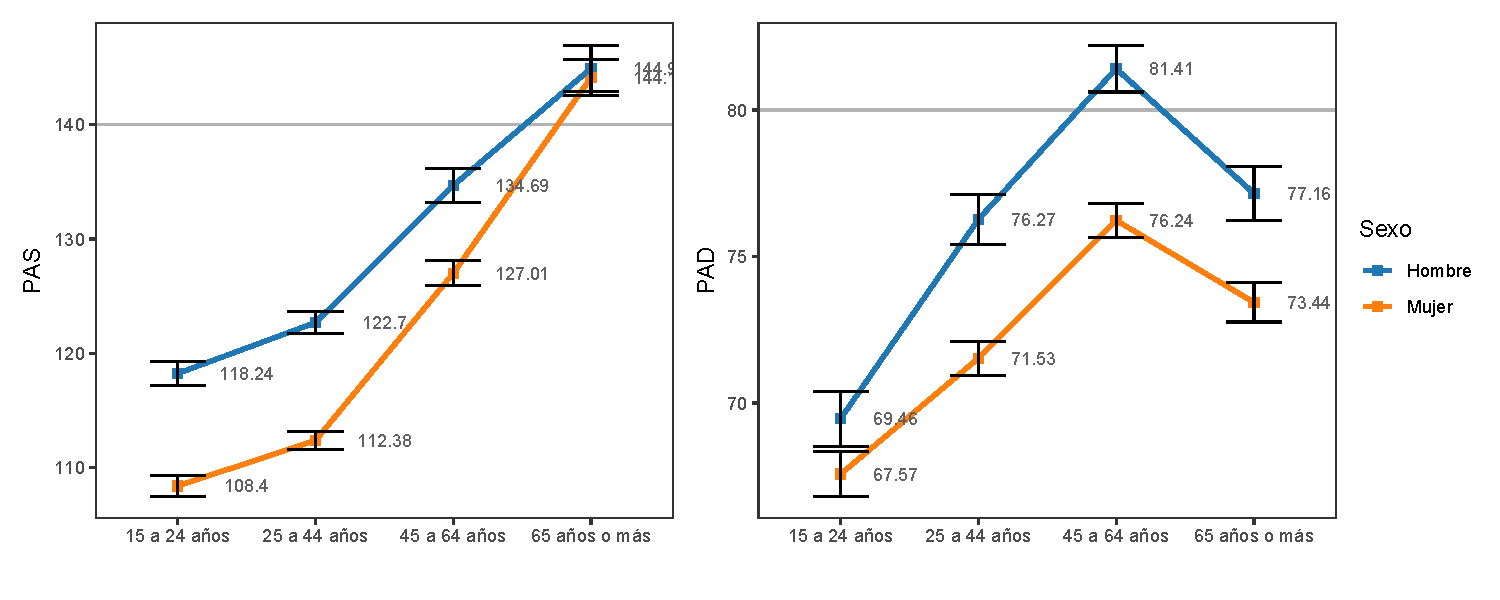
\includegraphics[scale = 0.6]{fig1.pdf}
        \caption{Presión Arterial por grupo de edad diferenciado por sexo}
        \label{fig:my_label}
    \end{figure}
\end{frame}

\subsection*{Prevalencia en sociodemográficas}
\begin{frame}{revalencia en sociodemográficas}
%%%%%% TABLA N %%%%%%%%%%%%%%%%%%%%%%%%%%%%%%%%%%%%%%%%%%%%%%%%%%%%%%%%
%%%%%%%%%%%%%%%%%%%%%%%%%%%%%%%%%%%%%%%%%%%%%%%%%%%%%%%%%%%%%%%%%%%%%%%
\begin{table}[]
\caption{\small Prevalencia FR}
    \centering
    
    \captionsetup[table]{labelformat=empty,skip=1pt}
\captionsetup[table]{labelformat=empty,skip=1pt}
\begin{tabular}{lccc}
\toprule
\textbf{Characteristic} & \textbf{No}, N = 3,503\textsuperscript{1} & \textbf{Sí}, N = 2,013\textsuperscript{1} & \textbf{p-value}\textsuperscript{2} \\ 
\midrule
N & 3,503 (64\%) & 2,013 (36\%) &  \\ 
\small Hombre & 1,111 (55\%) & 906 (45\%) &  <0.001\\ 
IMC & 27.6 (24.4, 31.4) & 29.5 (26.2, 33.2) & <0.001 \\ 
Edad & 42 (28, 58) & 60 (47, 71) & <0.001 \\ 
Zona &  &  & <0.001 \\ 
\-\hspace{5mm} \small Norte & 788 (69\%) & 353 (31\%) &  \\ 
\-\hspace{5mm} \small Metropolitana & 558 (67\%) & 273 (33\%) &  \\ 
\-\hspace{5mm} \small Centro-Sur & 1,287 (61\%) & 817 (39\%) &  \\ 
\-\hspace{5mm} \small Sur & 870 (60\%) & 570 (40\%) &  \\ 
Trabajando & 1,337 (66\%) & 693 (34\%) & 0.006 \\ 
 \bottomrule
\end{tabular}
\vspace{-5mm}
\begin{minipage}{\linewidth}
\textsuperscript{1}n (\%); Median (IQR) \\ 
\textsuperscript{2}Pearson\textquotesingle{}s Chi-squared test; Wilcoxon rank sum test \\ 
\end{minipage}

    \vspace{1ex}
    
    {\raggedright \small \textbf{Fuente:} Elaborado a partir de los datos de la Encuesta Nacional de Salud 2017 \par}
\end{table}
%%%%%%%%%%%%%%%%%%%%%%%%%%%%%%%%%%%%%%%%%%%%%%%%%%%%%%%%%%%%%%%%%%%%%%%
%%%%%%%%%%%%%%%%%%%%%%%%%%%%%%%%%%%%%%%%%%%%%%%%%%%%%%%%%%%%%%%%%%%%%%%
\end{frame}

% Categorías
\subsection*{Prevalencia patologías}
\begin{frame}{Prevalencia FR}
    %%%%%% TABLA N %%%%%%%%%%%%%%%%%%%%%%%%%%%%%%%%%%%%%%%%%%%%%%%%%%%%%%%%
%%%%%%%%%%%%%%%%%%%%%%%%%%%%%%%%%%%%%%%%%%%%%%%%%%%%%%%%%%%%%%%%%%%%%%%
\begin{table}[]
\caption{\small \small Prevalencia FR (patologías y estilo de vida)}
    \centering
    \small

    \captionsetup[table]{labelformat=empty,skip=1pt}
\begin{tabular}{lccc}
\toprule
\textbf{Characteristic} & \textbf{No}, N = 3,503\textsuperscript{1} & \textbf{Sí}, N = 2,013\textsuperscript{1} & \textbf{p-value}\textsuperscript{2} \\ 
\midrule
N & 3,503 (64\%) & 2,013 (36\%) &  \\ 
Categoría de edad &  &  & <0.001 \\ 
\-\hspace{5mm} \small 15 a 24 años & 668 (92\%) & 60 (8.2\%) &  \\ 
\-\hspace{5mm} \small 25 a 44 años & 1,224 (78\%) & 347 (22\%) &  \\ 
\-\hspace{5mm} \small 45 a 64 años & 1,047 (56\%) & 810 (44\%) &  \\ 
\-\hspace{5mm} \small 65 años o más & 564 (41\%) & 796 (59\%) &  \\ 
Categoría de IMC &  &  & <0.001 \\ 
\-\hspace{5mm} \small Peso insuficiente & 38 (73\%) & 14 (27\%) &  \\ 
\-\hspace{5mm} \small Normopeso & 975 (76\%) & 312 (24\%) &  \\ 
\-\hspace{5mm} \small Sobrepeso & 1,334 (64\%) & 752 (36\%) &  \\ 
\-\hspace{5mm} \small Obesidad & 1,139 (55\%) & 915 (45\%) &  \\ 
 \bottomrule
\end{tabular}
    \vspace{5mm}
    
    {\raggedright \small \textbf{Fuente:} Elaborado a partir de los datos de la Encuesta Nacional de Salud 2017 \par}
\end{table}
%%%%%%%%%%%%%%%%%%%%%%%%%%%%%%%%%%%%%%%%%%%%%%%%%%%%%%%%%%%%%%%%%%%%%%%
%%%%%%%%%%%%%%%%%%%%%%%%%%%%%%%%%%%%%%%%%%%%%%%%%%%%%%%%%%%%%%%%%%%%%%%
\end{frame}

\subsection*{Prevalencia patologías II}
\begin{frame}{Prevalencia FR}
    %%%%%% TABLA N %%%%%%%%%%%%%%%%%%%%%%%%%%%%%%%%%%%%%%%%%%%%%%%%%%%%%%%%
%%%%%%%%%%%%%%%%%%%%%%%%%%%%%%%%%%%%%%%%%%%%%%%%%%%%%%%%%%%%%%%%%%%%%%%
\begin{table}[]
\caption{\small Estadísticos descriptivos de las variables}
    \centering
    \small

    \captionsetup[table]{labelformat=empty,skip=1pt}
\begin{tabular}{lccc}
\toprule
\textbf{Characteristic} & \textbf{No}, N = 3,503\textsuperscript{1} & \textbf{Sí}, N = 2,013\textsuperscript{1} & \textbf{p-value}\textsuperscript{2} \\ 
\midrule
N & 3,503 (64\%) & 2,013 (36\%) &  \\ 
Hombre & 1,111 (55\%) & 906 (45\%) &  \\ 
Hipercolesterolemia & 564 (52\%) & 526 (48\%) & <0.001 \\
Diabetes & 409 (50\%) & 406 (50\%) & <0.001 \\ 
Fuma & 1,077 (69\%) & 483 (31\%) & <0.001 \\ 
Depresión & 789 (66\%) & 411 (34\%) & 0.068 \\ 
 \bottomrule
\end{tabular}
    \vspace{5mm}
    
    {\raggedright \small \textbf{Fuente:} Elaborado a partir de los datos de la Encuesta Nacional de Salud 2017 \par}
\end{table}
%%%%%%%%%%%%%%%%%%%%%%%%%%%%%%%%%%%%%%%%%%%%%%%%%%%%%%%%%%%%%%%%%%%%%%%
%%%%%%%%%%%%%%%%%%%%%%%%%%%%%%%%%%%%%%%%%%%%%%%%%%%%%%%%%%%%%%%%%%%%%%%
\end{frame}

\subsection*{Diabetes I}
\begin{frame}{Prevalencia: Diabetes}
    \begin{table}[]
\caption{\small Prevalencia: Diabetes}
    \centering
    \small

    \captionsetup[table]{labelformat=empty,skip=1pt}
\begin{tabular}{lccc}
\toprule
\textbf{Characteristic} & \textbf{No}, N = 3,503\textsuperscript{1} & \textbf{Sí}, N = 2,013\textsuperscript{1} & \textbf{p-value}\textsuperscript{2} \\ 
\midrule
N & 3,503 (64\%) & 2,013 (36\%) &  \\ 
Diabetes & 409 (50\%) & 406 (50\%) & <0.001 \\ 
 \bottomrule
\end{tabular}
    \vspace{5mm}
    
    {\raggedright \small \textbf{Fuente:} Elaborado a partir de los datos de la Encuesta Nacional de Salud 2017 \par}
\end{table}
\end{frame}

\subsection*{Diabetes II}
\begin{frame}{Presión Arterial y Diabetes}
    \begin{figure}
        \centering
        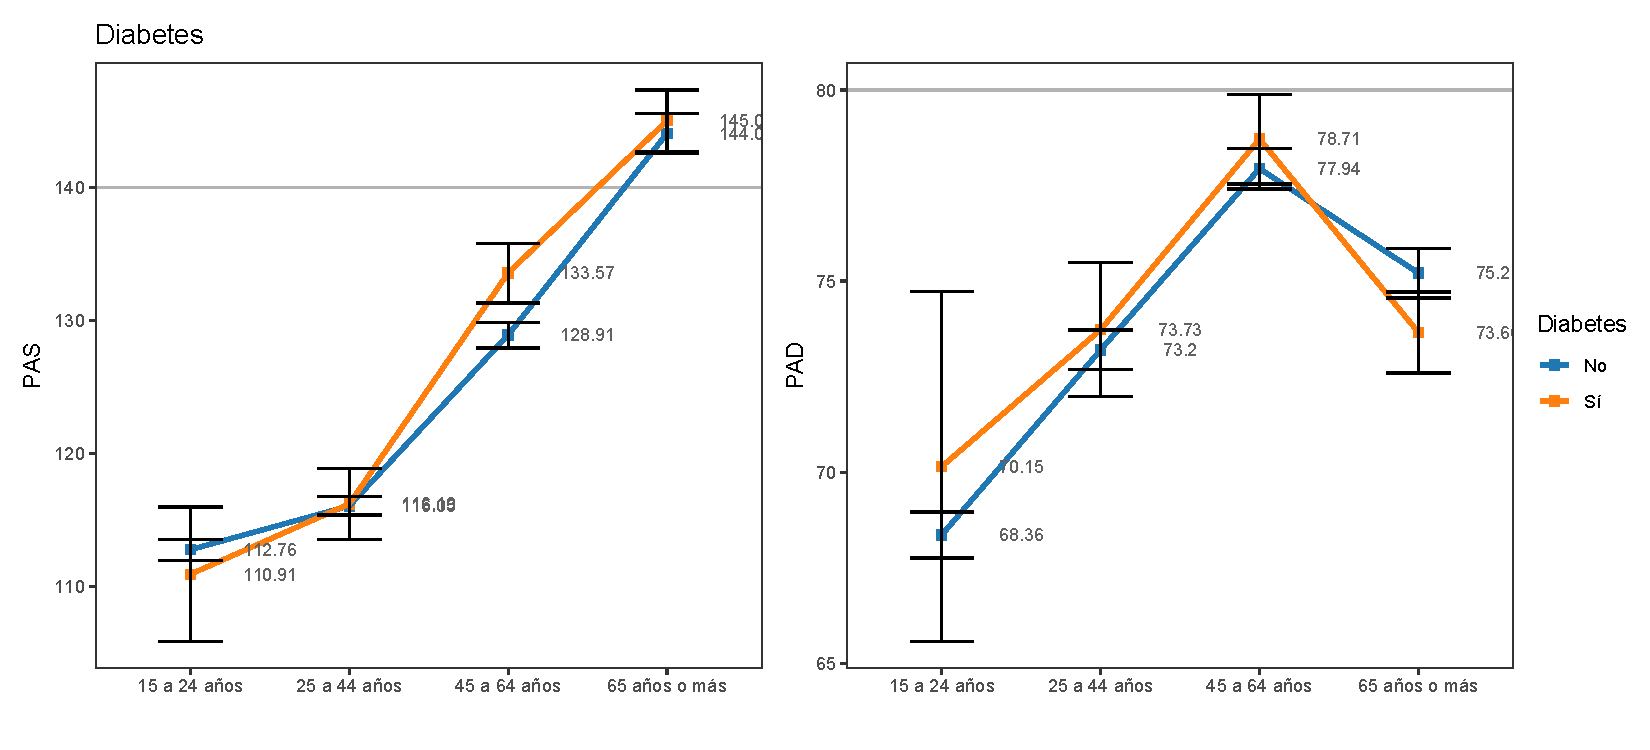
\includegraphics[scale = .5]{img/fig2.pdf}
        \caption{PA y diabetes}
        \label{fig:my_label}
    \end{figure}
\end{frame}


\subsection*{Fumar}
\begin{frame}{Prevalencia: Fumar}
    \begin{table}[]
\caption{\small Estadísticos descriptivos de las variables}
    \centering
    \small

    \captionsetup[table]{labelformat=empty,skip=1pt}
\begin{tabular}{lccc}
\toprule
\textbf{Characteristic} & \textbf{No}, N = 3,503\textsuperscript{1} & \textbf{Sí}, N = 2,013\textsuperscript{1} & \textbf{p-value}\textsuperscript{2} \\ 
\midrule
N & 3,503 (64\%) & 2,013 (36\%) &  \\ 
Fuma & 1,077 (69\%) & 483 (31\%) & <0.001 \\ 
 \bottomrule
\end{tabular}
    \vspace{5mm}
    
    {\raggedright \small \textbf{Fuente:} Elaborado a partir de los datos de la Encuesta Nacional de Salud 2017 \par}
\end{table}
\end{frame}

\subsection*{Fumar II}
\begin{frame}{Presión Arterial y Diabetes}
    \begin{figure}
        \centering
        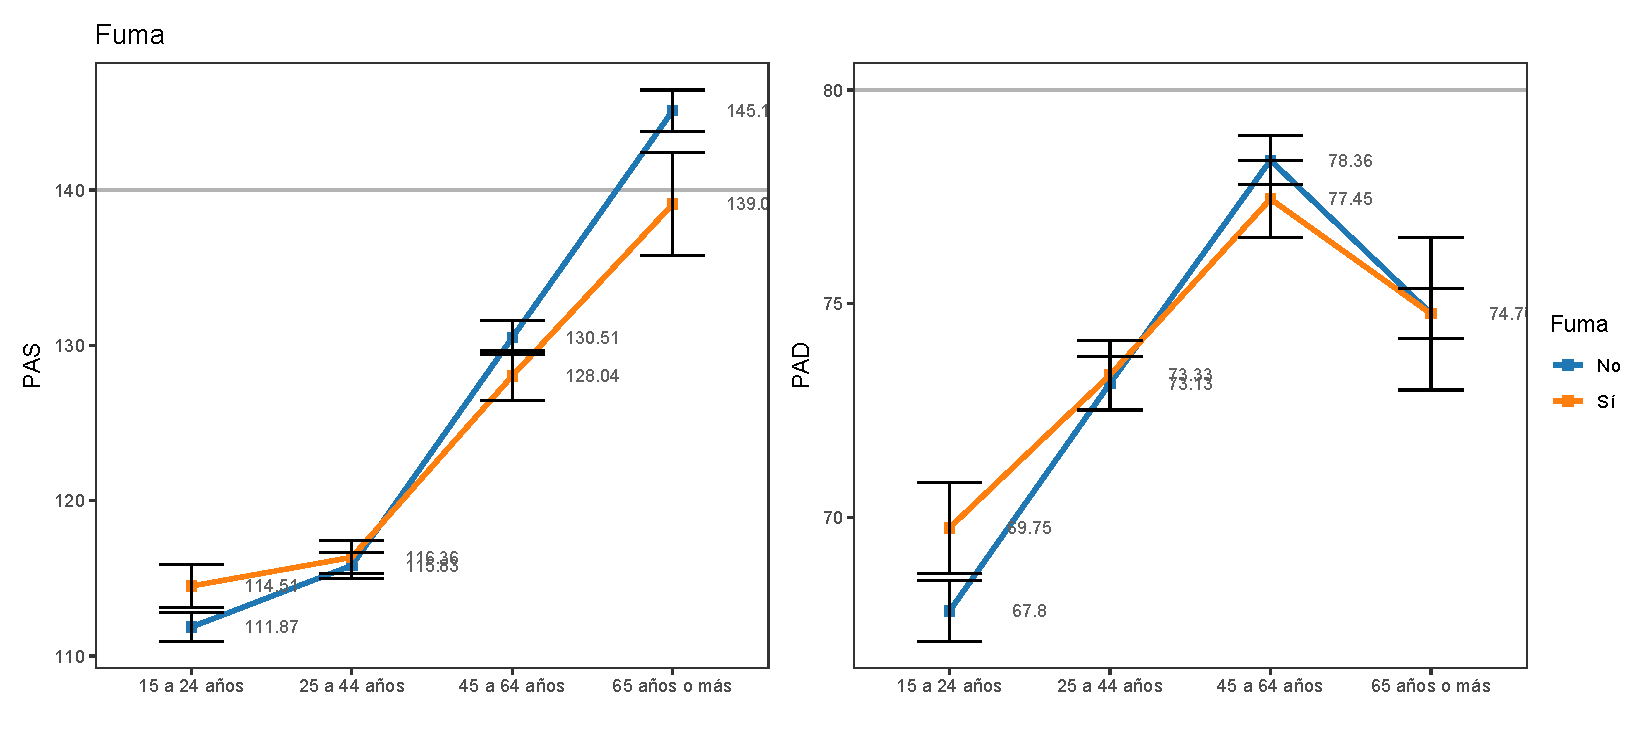
\includegraphics[scale = .5]{img/fig3.pdf}
        \caption{PA y fumadores}
        \label{fig:my_label}
    \end{figure}
\end{frame}

\subsection*{Prevalencia: IMC > 25}
\begin{frame}{Prevalencia: IMC mayor a 25 kg/$m^2$}
    \begin{table}[]
\caption{\small \small Prevalencia FR (patologías y estilo de vida)}
    \centering
    \small

    \captionsetup[table]{labelformat=empty,skip=1pt}
\begin{tabular}{lccc}
\toprule
\textbf{Characteristic} & \textbf{No}, N = 3,503\textsuperscript{1} & \textbf{Sí}, N = 2,013\textsuperscript{1} & \textbf{p-value}\textsuperscript{2} \\ 
\midrule
N & 3,503 (64$\%$) & 2,013 (36$\%$) &  \\ 
Categoría de IMC &  &  & <0.001 \\ 
\-\hspace{5mm} \small Peso insuficiente & 38 (73$\%$) & 14 (27$\%$) &  \\ 
\-\hspace{5mm} \small Normopeso & 975 (76$\%$) & 312 (24$\%$) &  \\ 
\-\hspace{5mm} \small Sobrepeso & 1,334 (64$\%$) & 752 (36$\%$) &  \\ 
\-\hspace{5mm} \small Obesidad & 1,139 (55$\%$) & 915 (45$\%$) &  \\ 
 \bottomrule
\end{tabular}
    \vspace{5mm}
    
    {\raggedright \small \textbf{Fuente:} Elaborado a partir de los datos de la Encuesta Nacional de Salud 2017 \par}
\end{table}
\end{frame}

\subsection*{Presión arterial IMC > 25 II}
\begin{frame}{Presión Arterial e IMC mayor a 25 kg/$m^2$}
    \begin{figure}
        \centering
        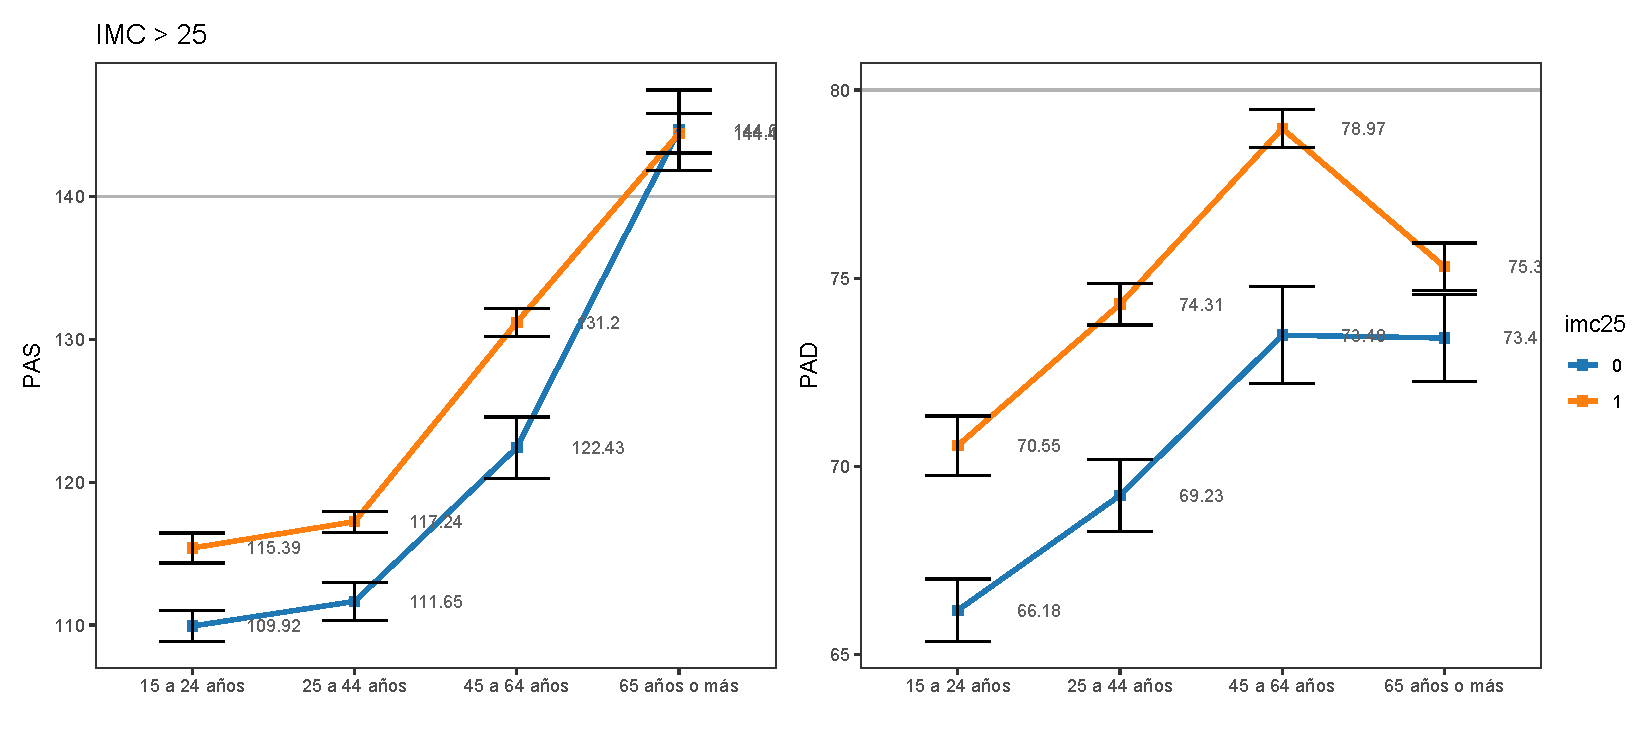
\includegraphics[scale = .5]{img/fig4.pdf}
        \caption{Presión arterial e IMC mayor a 25}
        \label{fig:my_label}
    \end{figure}
\end{frame}

\subsection*{Hipercolesterolemia}
\begin{frame}{Prevalencia: Colesterol Alto (Hipercolesterolemia)}
    \begin{table}[]
\caption{\small Prevalencia: Colesterol Alto}
    \centering
    \small

    \captionsetup[table]{labelformat=empty,skip=1pt}
\begin{tabular}{lccc}
\toprule
\textbf{Characteristic} & \textbf{No}, N = 3,503\textsuperscript{1} & \textbf{Sí}, N = 2,013\textsuperscript{1} & \textbf{p-value}\textsuperscript{2} \\ 
\midrule
N & 3,503 (64\%) & 2,013 (36\%) &  \\ 
Hipercolesterolemia & 564 (52\%) & 526 (48\%) & <0.001 \\
 \bottomrule
\end{tabular}
    \vspace{5mm}
    
    {\raggedright \small \textbf{Fuente:} Elaborado a partir de los datos de la Encuesta Nacional de Salud 2017 \par}
\end{table}
\end{frame}

\subsection*{Hipercolesterolemia II}
\begin{frame}{Presión Arterial y Diabetes}
    \begin{figure}
        \centering
        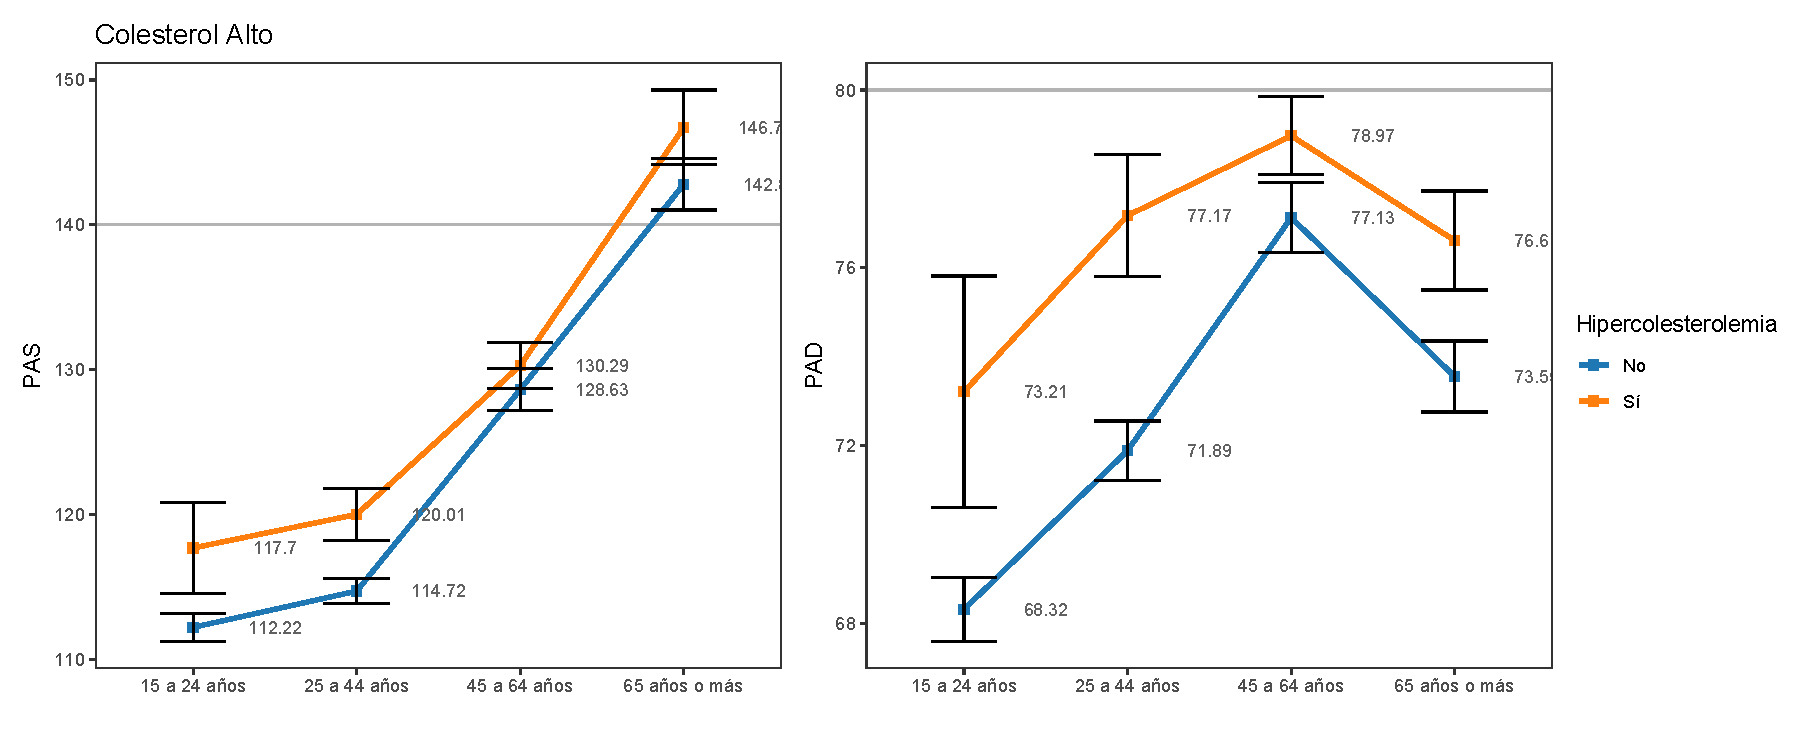
\includegraphics[scale = .5]{img/fig5.pdf}
        \caption{PA y diabetes}
        \label{fig:my_label}
    \end{figure}
\end{frame}

\subsection*{Depresión}
\begin{frame}{Prevalencia: Depresión}
    \begin{table}[]
\caption{\small ´Prevalencia: Depresión}
    \centering
    \small

    \captionsetup[table]{labelformat=empty,skip=1pt}
\begin{tabular}{lccc}
\toprule
\textbf{Characteristic} & \textbf{No}, N = 3,503\textsuperscript{1} & \textbf{Sí}, N = 2,013\textsuperscript{1} & \textbf{p-value}\textsuperscript{2} \\ 
\midrule
N & 3,503 (64\%) & 2,013 (36\%) &  \\ 
Depresión & 789 (66\%) & 411 (34\%) & 0.068 \\ 
 \bottomrule
\end{tabular}
    \vspace{5mm}
    
    {\raggedright \small \textbf{Fuente:} Elaborado a partir de los datos de la Encuesta Nacional de Salud 2017 \par}
\end{table}
\end{frame}

\subsection*{Depresión II}
\begin{frame}{Presión Arterial y Depresión}
    \begin{figure}
        \centering
        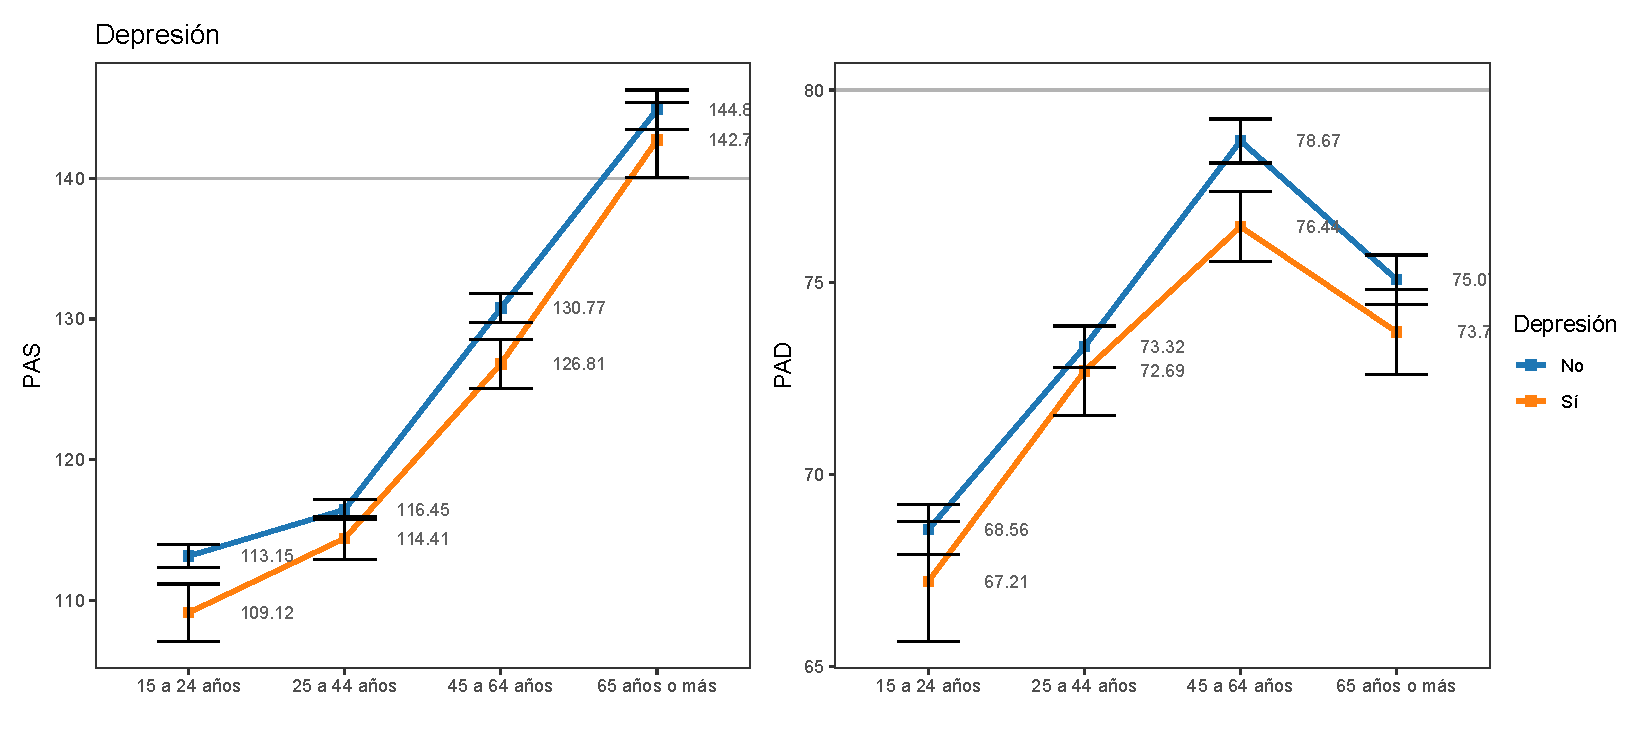
\includegraphics[scale = .5]{img/fig6.pdf}
        \caption{PA y diabetes}
        \label{fig:my_label}
    \end{figure}
\end{frame}

\subsection*{Odds Ratio}
\begin{frame}{Odds Ratio}
    \begin{table}[b]
\caption{\small Odds Ratio Factores de Riesgo de HTA}
    \centering
    \small
\begin{tabular}{lrcr}
\toprule
  & OR & IC95\% & valor-p\\
\midrule
Categoría de edad\\
\-\hspace{5mm} \small  15 a 24 años (ref) & 1.00 & & <0.001\\
\-\hspace{5mm} \small   25 a 44 años & 3.16 & [2.36-4.22] & <0.001\\
\-\hspace{5mm} \small   45 a 64 años & 8.61 & [6.51-11.39] & <0.001\\
\-\hspace{5mm} \small   65 años o más & 15.71 & [11.81-20.90] & <0.001\\
\addlinespace
Categoría de IMC\\
\-\hspace{5mm} \small   Peso insuficiente (ref) & 1.00 &  & 0.66\\
\-\hspace{5mm} \small   Normopeso & 0.87 & [0.46-1.62] & 0.18\\
\-\hspace{5mm} \small  Sobrepeso & 1.53 & [0.82-2.84] & 0.01\\
\-\hspace{5mm} \small   Obesidad & 2.18 & [1.17-4.05] & <0.001\\
\bottomrule
\end{tabular}
    \vspace{1ex}
    
    {\raggedright \small \textbf{Fuente:} Elaborado a partir de los datos de la Encuesta Nacional de Salud 2017 \par}
\end{table}
\end{frame}



\subsection*{Odds Ratio II}
\begin{frame}{Odds Ratio}
    \begin{table}[b]
\caption{\small Odds Ratio Factores de Riesgo de HTA}
    \centering
    \small
\begin{tabular}{lrcr}
\toprule
  & OR & IC95\% & valor-p\\
\midrule
Hombre = 1 & 1.76 & [1.57-1.97] & <0.001\\
Diabetes & 1.91 & [1.65-2.22] & <0.001\\
\addlinespace
Fuma & 0.71 & [0.63-0.81] & <0.001\\
\addlinespace
Hipercolesterolemia & 2.08 & [1.80-2.40] & <0.001\\
\bottomrule
\end{tabular}
    \vspace{1ex}
    
    {\raggedright \small \textbf{Fuente:} Elaborado a partir de los datos de la Encuesta Nacional de Salud 2017 \par}
\end{table}
\end{frame}

\section{Conclusión y comentarios finales}

\begin{frame}{Conclusiones y comentarios finales}
    \textcolor{preambulo}{\textbf{Prevalencia de hipertensión}}
    \begin{itemize}
    \pro Más de un tercio de la muestra representativa recibiría un diagnóstico de hipertensión
    \pro Apenas un décimo reconoce conocer su posible diagnóstico
    \end{itemize}

\textcolor{preambulo}{\textbf{Prevalencia en factores de riesgo}}
\begin{itemize}
    \pro Cerca de la mitad de personas que padecían 
    \pro Se demostró que ser hombre
    \pro Lamentablemente, existirán elementos de la patogénesis de la depresión que impidan relacionarlo con la hipertensión, pero debemos aumentar el enfoque.
\end{itemize}

\textit{La investigación biomédica como elemento clave en la modernidad}
\end{frame}

\begin{frame}{Conclusiones y comentarios finales II}
\textcolor{preambulo}{\textbf{Sobre el compromiso social de la ciencia}}
    \begin{itemize}
    \pro No fue fácil llegar a este grado de sofisticación de diagnóstico!
    \pro Políticas Públicas basadas en evidencias para impedir discusiones que no aportan nada a la democracia
    \pro Hacer que el paciente tome decisiones informado sobre su bienestar
    \pro Todavía falta mucho: apenas un décimo reconoce conocer su posible diagnóstico
\end{itemize}
\end{frame}

\begin{frame}{}
    \vfill
    \centering
    \Huge
    ¡Gracias!\\
    \textcolor{preambulo}{¿Preguntas?}
    \vfill
\end{frame}

\end{document}
